\documentclass[9pt,a4paper,twocolumn,twoside]{tau-class/tau}
\usepackage[english]{babel}
\usepackage[spanish,es-nodecimaldot,es-noindentfirst]{babel}

\addbibresource{referencias.bib}

%----------------------------------------------------------
% Title & Authors/Affiliations
%----------------------------------------------------------

\doctype{Seminario de Heur\'isticas de Optimizaci\'on Combinatoria 2027-1}
\title{Recocido simulado por aceptaci\'on de umbrales para una variante del problema del agente viajero}

%----------------------------------------------------------

\author[]{Lara Guill\'en Gilabert\\

\small{En colaboraci\'on el grupo del Seminario de Heur\'isticas de Optimizaci\'on Combinatoria. Quiero dar mis m\'as sincero agradecimiento a las personas que durante el desarrollo de este proyecto intercambiaron conmigo sus ideas y resultados, en especial a Wendy S\'anchez Cort\'es, Manuel Ianluck Rojo Peña y Carlos Cabrera Ram\'irez. Este \'ultimo fue quien tuvo la generosidad de echarme una mano con la generaci\'on de mapas que se encuentran en este documento.}}


%----------------------------------------------------------
% Document-, Footer- information
%----------------------------------------------------------


%----------------------------------------------------------

\footinfo{Recocido Simulado}
\theday{\today}
\organization{Seminario de Heur\'isticas de Optimizaci\'on Combinatoria}
\leadauthor{Lara Guill\'en}

% ==============================================================================
% ABSTRACT
% ==============================================================================



\begin{abstract}    
En este trabajo se presenta el diseño, implementación y evaluación experimental de un programa en orientado a la resolución de la variante del Problema del Agente Viajero sobre camimos hamiltonianos mediante la heur\'istica de recocido simulado por aceptaci\'on de umbrales (Threshold Accepting, Dueck \& Scheuer). La implementaci\'on escrita en Java evalúa el costo de cada solución de forma eficiente y permite reproducir cualquier ejecuci\'on a partir de su semilla. Se mejoró la forma en que el algoritmo explora soluciones vecinas, permitiendo explorar el espacio de b\'usqueda de forma m\'as precisa.\\

\end{abstract}

%----------------------------------------------------------

\begin{document}
		
    \maketitle 
    \thispagestyle{firststyle}
    
% ==============================================================================
% 1. INTRODUCCIÓN
% ==============================================================================

\section{Introducci\'on}

    \taustart{L}a optimizaci\'on combinatoria sobre gr\'aficas constituye uno de los n\'ucleos te\'oricos m\'as importantes en las ciencias de la computaci\'on, debido a sus aplicaciones pr\'acticas. El Problema del Agente Viajero (TSP, Traveler Salesman Problem por sus siglas en ingl\'es) destaca por ser uno de los problemas NP-dif\'icil m\'as estudiados en el \'area, cuyas variantes de optimizaci\'on sobre gr\'aficas ponderadas generales resultan intratables mediante algoritmos exactos. Cuenta con aplicaciones directas en \'areas como en log\'istica y reparto para establecer rutas \'optimas, en gen\'omica para la secuenciaci\'on de ADN o en manufactura de circuitos para decidir el recorrido que realizan las m\'aquinas que los taladran. Por ello, el diseño de heur\'isticas y m\'etodos estoc\'asticos se vuelve imperativo.\\
    

    En este trabajo se propone e implementa una heur\'istica de optimizaci\'on combinatoria basada en Aceptaci\'on por Umbrales (\textit{Threshold Accepting}, TA), originalmente desarrollada por Dueck y Scheuer~\cite{dueck1990threshold}. El algortimo que se presenta es una variante determinista del recocido simulado que resuelve la variante del Problema del Agente Viajero sobre caminos hamiltonianos: dado un conjunto de ciudades y las distancias entre ellas, se busca la ruta de menor costo que las visite todas. El tamaño de b\'usqueda para esta variante respecto a $n$ ciudades es de $\frac{n!}{2}$ caminos distintos posibles, sin distinci\'on de direcci\'on.\\
    
    
    La idea del algoritmo se basa en la optimización local: se parte de una ruta inicial y se proponen pequeños cambios locales, aceptando aquellos que no empeoren significativamente el costo actual al comenzar con umbrales altos y reducirlos gradualmente. Esto divide al algoritmo en una etapa de exploración del espacio de soluciones, donde frecuentemente se aceptan rutas peores, y una etapa de explotación, donde la exigencia aumenta hasta converger a una solución de bajo costo. No se puede asegurar que la soluci\'on encontrada es la \'optima; se busca que sea lo suficientemente buena y pueda calcularse en pocos minutos o segundos.\\

% ==============================================================================
% 2. DEFINICIÓN DEL PROBLEMA
% ==============================================================================
\section{Problema del Agente Viajero sobre caminos hamiltonianos}label{sec:problema}

    \subsection{Formalizaci\'on del espacio de b\'usqueda}

        Sea $S$ el conjunto de $k$ ciudades que forman parte de la instancia a tratar, y sea $G=(S,E)$ la gráfica que $S$ induce a partir de la base de datos disponible. Cada arista $(u, v) \in E$ posee un peso asociado $w(u, v) > 0$, correspondiente a la distancia real de traslado entre ambas ciudades. Dado que no todo par de vértices cuenta con una conexión directa, $G$ es, en el caso general, una gráfica no completa.\\


        Una solución candidata $P$ se define como una permutación de los elementos de $S$; es decir, una secuencia $(P_1, P_2, \dots, P_k)$ que visita cada ciudad exactamente una vez. Al tratarse de una variante sobre caminos hamiltonianos, nunca se regresa al v\'ertice de origen. El costo se eval\'ua \'unciamente a lo largo de las $k-1$ conexiones consecutivas $(P_i, P_{i+1})$.

    \subsection{M\'etrica de distancia y funci\'on de costo penalizada}

        Para la evaluaci\'on de una permutaci\'on sobre una gr\'afica, el modelo se basa en las siguientes definiciones:

        \begin{itemize}
            \item \textbf{Distancia natural, $d(u, v)$:} Distancia geográfica entre dos ciudades calculada mediante la fórmula \textit{Haversine} a partir de sus coordenadas. Esta función se puede calcular independientemente de si la arista $(u, v)$ pertenece o no a $E$.\\
            
            \item \textbf{Distancia máxima, $\max_d(S)$:} Cota superior de los pesos asociados a las aristas válidas de la instancia:
            \begin{equation}
                \max_d(S) = \max_{(u, v) \in E} w(u, v)
            \end{equation}\\
            
            \item \textbf{Peso aumentado, $w_S(u, v)$:} Penalización estricta por conexi\'on ausente entre ciudades:\\
            \begin{equation}
                w_S(u, v) = \begin{cases} 
                    w(u, v) & \text{si } (u, v) \in E \\ 
                    d(u, v) \times \max_d(S) & \text{si } (u, v) \notin E 
                \end{cases}
            \end{equation}\\

            Cuando la arista existe en $G$, se toma su peso real; de lo contrario, se impone un castigo al multiplicar su distancia natural por el valor máximo presente en la instancia. Esta penalización supera ampliamente cualquier distancia admisible, superando por varios \'ordenes de magnitud el valor de las distancias reales. Gracias a esta penalizaci\'on es que se puede discernir f\'acilmente soluciones factibles de aquellas que no lo son. \\
            
            
            \item \textbf{Factor de normalización, $N(S)$:} Suma de los $k - 1$ pesos válidos más grandes presentes en $G$. Permite comparar el comportamiento del algoritmo sobre instancias de distinta cardinalidad.\\
            
            \item \textbf{Costo normalizado, $f(P)$:} La función objetivo a minimizar queda formulada como:
            \begin{equation}
                f(P) = \frac{1}{N(S)} \sum_{i=1}^{k-1} w_S(P_i, P_{i+1})
            \end{equation}
        \end{itemize}

    \subsection{Criterio anal\'itico de factibilidad}

		Una permutación $P$ se clasifica como \textbf{factible} si representa un camino hamiltoniano válido en $G$; es decir, si cada transición consecutiva satisface $(P_i, P_{i+1}) \in E$. Por la construcción de $N(S)$ y la severidad del peso aumentado $w_S$, la factibilidad de una ruta se determina de manera exacta y sin costo computacional adicional a partir de su evaluación numérica:
        
        \begin{equation}
            f(P) \le 1 \iff P \text{ es factible}
        \end{equation}
        
        Si una permutación contiene al menos una arista ausente, el término de penalización correspondiente sobrepasa individualmente el valor de $N(S)$, provocando que $f(P) > 1$.\\

        El espacio de b\'usqueda comprende $\frac{n!}{2}$ rutas posibles, donde $n$ es el n\'umero de ciudades de la instancia a tratar. Cuando $n$ crece, la evaluaci\'on exhaustiva se vuelve inviable. Para guiar la optimización local, se introduce la noción de solución vecina: una permutación $P'$ derivada de $P$ mediante el intercambio de un par de aristas. Por tanto, lo que se busca es encontrar una permutaci\'on que minimice $f(P)$, que por supuesto sea una trayectoria factible en $G$.



% ==============================================================================
% 3. HEURÍSTICA PROPUESTA
% ==============================================================================

\section{Heur\'istica: Recocido Simulado de Aceptaci\'on por Umbrales }\label{sec:heuristica}

Dado el crecimiento factorial del espacio de soluciones, es natural buscar una heur\'istica que sea capaz de aproximarnos a una buena soluci\'on; una que minimice el costo. En metalurgia, el recocido (\textit{annealing}) es una t\'ecnica de tratamiento t\'ecnico aplicada a metales: se calienta por encima de una temperatura cr\'itica para luego dejarse enfriar de manera lenta y controlada. Cuando la temperatura es alta, las part\'iculas del material poseen una energ\'ia cin\'etica muy alta que les permite moverse de manera m\'as libre por el espacio. Conforme la temperatura desciende, la movilidad se ve reducida y los \'atomos se ven obligados a organizarse en estados de menor energ\'ia, haciendo que el sistema termine con configuraciones estables de energ\'ia m\'inima global.\\

Scott Kirkpatrick, C. Daniel Gelatt y Mario Vecchi retomaron la idea del recocido en metalurgia para plantear un an\'alogo donde tambi\'en se busca encontrar la configuraci\'on de costo m\'inimo. Propusieron sustituir la función de energía del sistema físico por la función objetivo de costo, y parametrizar el proceso con una temperatura de control~\cite{kirkpatrick1983optimization}. M\'as adelante, Dueck y Scheuer cuestionaron el c\'alculo probabil\'istico para escapar de m\'inimos locales. Propusieron la Aceptaci\'on por Umbrales como alternativa~\cite{dueck1990threshold} con una regla de aceptaci\'on determinista:

\[
\text{aceptar } s' \iff f(s') \le f(s) + T,
\]


    \subsection{B\'usqueda local}

    En cada iteración se genera un vecino $s'$ de la solución actual $s$ mediante una modificación local mínima del camino, y se acepta si su costo no excede el de $s$ en más que el umbral $T$ actual. $T$ puede iniciar siendo alta, permitiendo aceptar movimientos que empeoran la solución, lo que evita quedar atrapado en m\'inimos locales desde temprano. Se parte desde $T_0$ y se reduce mediante un factor de enfriamiento $\varphi \in (0,1)$, que suele ser cercano a $1$ para un enfriamiento m\'as lento.

    \subsection{Vecinidad}
    El operador de vecindad usado inicialmente intercambiaba dos posiciones del camino elegidas al azar, alterando hasta cuatro aristas por movimiento. Se sustituyó por una reversión de segmento~\cite{croes1958method}: se eligen dos índices $i<j$ al azar y se invierte el subcamino entre ellos, lo que altera a lo más dos aristas, que son esenciamente las que conectan el segmento invertido con el resto del camino. Las aristas internas del segmento son las mismas recorridas en sentido contrario y, al ser la matriz de pesos de $G$ simétrica, su suma no cambia. Un cruce en la ruta siempre es subóptimo bajo una métrica geométrica, y la reversión lo elimina en un solo paso, mientras que el intercambio solo llega a la misma configuración pasando por estados intermedios que el umbral puede rechazar.

    \subsection{Convergencia y terminaci\'on}
    El algoritmo no garantiza optimalidad. Termina cuando $T \le \varepsilon$. Para evitar que una combinación de parámetros que no llega a enfriarse deje el programa corriendo indefinidamente, tambi\'en se introdujeron un n\'umero m\'aximo de intentos. El resultado reportado es la mejor solución vista a lo largo de toda la ejecuci\'on.



% ==============================================================================
% 4. DISEÑO DE LA SOLUCIÓN
% ==============================================================================
\section{Diseño de la Solución}\label{sec:diseno}

El sistema se organiza en cuatro capas con dependencias en un solo sentido: \inlinecode{data} (lectura de la base de datos), \inlinecode{domain} (la instancia y las soluciones), \inlinecode{heuristic} (el algoritmo) y \inlinecode{experiment} (los barridos de semillas), coordinadas por \inlinecode{app.Main}.


    \subsection{Arquitectura del proyecto}

    El proyecto se organiza en seis paquetes bajo \inlinecode{mx.unam.fciencias.tsp}:

    \begin{verbatim}
mx.unam.fciencias.tsp
|-- data        DatabaseBuilder, GraphDao, InstanceReader,
|               DataException
|-- domain      HaversineDistance, Instance, Solution,
|               Route, CostTrace, InvalidInstanceException,
|               InvalidRouteException
|-- exhaustive  Permutation
|-- heuristic   SimulatedAnnealing, Parameters, Outcome,
|               StopReason, CostListener
|-- experiment  SeedSweep, Trial, TrialWriter
|-- app         Main, Configuration, PropertiesReader,
                ParameterException
    \end{verbatim}

    \subsection{Estructuras de Datos Principales}

    Una instancia mantiene \textit{}{dos} matrices $k\times k$: \inlinecode{weights}, con el peso real o $0.0$ si la arista está ausente, y \inlinecode{augmented}, con $w_S(u,v)$ precalculada. Mantener ambas evita recalcular la distancia Haversine de cada arista ausente en cada evaluación de costo.\\

    El mapeo de identificador de ciudad a posición dentro de la instancia se resuelve con un arreglo indexado por \inlinecode{id}$-1$.\\
    
    Una solución se representa como un arreglo de $k$ enteros, que es una permutación de posiciones,junto con su costo ya calculado, para no tener que recalcularlo en cada consulta.

    \subsection{Flujo del programa}

    Una ejecuci\'on atraviesa los paquetes en este orden:\\
    \begin{enumerate}
      \item \inlinecode{app.Main} lee la configuración (\inlinecode{Configuration}, \inlinecode{PropertiesReader}) desde un \inlinecode{.properties}.
      \item \inlinecode{data.DatabaseBuilder} construye el \inlinecode{.db} a partir del \inlinecode{.sql} si aún no existe, y lo reutiliza en caso contrario.
      \item \inlinecode{data.InstanceReader} lee el \inlinecode{.tsp} y produce los \textit{id's} de $S$ en el orden del archivo.
      \item \inlinecode{data.GraphDao} traduce esos ids a posiciones y entrega la subgr\'afica inducida por $S$: la matriz de pesos y las coordenadas.
      \item Con esos arreglos se construye una \inlinecode{domain.Instance}: valida sus invariantes, y precalcula \inlinecode{maxWeight()}, \inlinecode{normalizer()} y la matriz de pesos aumentados.
      \item A partir de la \inlinecode{Instance} se resuelve el problema por uno de dos caminos, mutuamente ajenos:
      \begin{itemize}
        \item \inlinecode{exhaustive.Permutation} enumera las $k!$ ordenaciones y devuelve la óptima, solo viable para $k$ pequeña.
        \item \inlinecode{heuristic.SimulatedAnnealing.bestRoute} ejecuta los procedimientos 1 a 5 (lote, corrida por umbrales, búsqueda de temperatura inicial) sobre objetos \inlinecode{Route}, guiada por \inlinecode{Parameters}, y devuelve un \inlinecode{Outcome} con la mejor \inlinecode{Route} vista, su costo y el \inlinecode{StopReason}.
      \end{itemize}
      \item Para experimentación, \inlinecode{experiment.SeedSweep} repite el paso anterior una vez por semilla sobre la misma \inlinecode{Instance}, en paralelo, y \inlinecode{TrialWriter} acumula los pares \inlinecode{(seed, cost)} en un CSV.
      \item \inlinecode{Main} imprime el camino resultante (traducido de vuelta a ids de ciudad) y, en modo verboso, la traza de costos vía \inlinecode{CostListener}.
    \end{enumerate}    

    \subsection{Procedimientos de la heur\'istica}
    El recocido simulado se divide en cinco procedimientos: el lote (\inlinecode{batch}), la ejecuci\'on por umbrales (\inlinecode{bestRoute}), la búsqueda de temperatura inicial (\inlinecode{temperatureSearch}), el porcentaje de aceptación (\inlinecode{countsAccepted}) y la búsqueda binaria (\inlinecode{binaryTemperatureSearch})~\cite{pelaez-notas}.

    \subsubsection{Lotes}

    Genera vecinos hasta aceptar $L$ soluciones o agotar el n\'umero m\'aximo de intentos por lote. Acepta de forma determinista cuando $f(s') \leq f(s) + T$ y devuelve el promedio de las aceptadas.
    
		\begin{code}
			\inputminted{java}{Lotes.java}
            \caption{M\'etodo \inlinecode{batch} para calcular lotes.}
			\label{lst:batch}
		\end{code}

        \subsubsection{Umbrales}
    
        Para cada temperatura, se repiten lotes hasta que ya no se mejoren. Se considera que en ese momento se alcanz\'o el equilibrio t\'ermico. Enfr\'ia $T *=\varphi$ y termina al alcanzar $\varepsilon$ o agotar el n\'umero total de intentos.
        
    		\begin{code}
    			\inputminted{java}{Lotes.java}
                \caption{Ciclo de \inlinecode{bestRoute}.}
    			\label{lst:batch}
    		\end{code}
    
        \subsubsection{Temperatura inicial}
        Calcula el doble o la mitad de $T$ hasta llegar la aceptaci\'on objetivo, y luego llama a la b\'suqueda binaria.
        
        \subsubsection{Porcentaje de aceptaci\'on}
        Camina $L$ pasos una temperatura fija y mide qu\'e fracci\'on fue aceptada.
    
        \subsubsection{B\'usqueda binaria para la temperatura}
        Encuentra la temperatura cuya fracci\'on de aceptaci\'on iguala el objetivo.

    \subsection{An\'alsis con Python}
    Adicionalmente, se agregan en el proyecto dos \textit{scripts} realizados en Python con el fin de analizar los resultados de las ejecuciones y generar las gr\'aficas mostradas más adelante.

    \subsubsection{\inlinecode{feasible.py}}


Toma uno o varios CSV de barrido de semillas y por cada uno filtra las corridas factibles, usando el mismo umbral que la propiedad de factibilidad $\Rightarrow f(P) \le 1$: (\inlinecode{FEASIBLE = 1.0}), y reporta qué fracción de las corridas lo cumplió. Además calcula estadísticas de resumen sobre las factibles: mejor, mediana, promedio, peor y desviación estándar. Genera un histograma de los costos factibles.


    
    \subsubsection{\inlinecode{plot.py}}
Grafica la traza de una única ejecución. Toma el CSV \inlinecode{evaluations,cost} que produce \inlinecode{CostListener} en modo verboso como una curva, que genera una gráfica de costo aceptado contra número de evaluaciones. 
% ==============================================================================
% 5. DETALLES DE IMPLEMENTACIÓN
% ==============================================================================
\section{DETALLES DE IMPLEMENTACIÓN}

\begin{itemize}
    \item \textbf{Lenguaje y compilación:} Java 21, compilado y empaquetado con Maven 3.8.7. Las pruebas usan JUnit~5.11.4; la lectura de la base de datos usa \inlinecode{sqlite-jdbc}~3.50.1.0. El empaquetado produce un \emph{jar} ejecutable autocontenido mediante \inlinecode{maven-shade-plugin}.\\
    
    \item \textbf{Reproducibilidad:} una única instancia de \inlinecode{java.util.Random},con una semilla explícita, se pasa por referencia. Ninguna estructura cuyo orden de iteración dependa del \textit{hash code} interviene en el cálculo, de modo que la misma semilla produce exactamente los mismos resultados en cualquier ejecución.\\
    
    \item \textbf{Evaluación incremental de costo:} el costo de un vecino no se recalcula desde cero. Como una reversión de segmento altera a lo más dos aristas del camino, el nuevo costo se obtiene sumando al costo actual la diferencia entre esas dos aristas antes y después del movimiento, dividida entre el normalizador.\\
    
    \item \textbf{Paralelización:} el barrido de semillas independientes (múltiples ejecuciones del mismo algoritmo sobre la misma instancia, cada una con su propia semilla) se ejecuta sobre un \textit{thread pool} de tamaño configurable, con una escritura sincronizada a un único archivo de resultados para no perder ejecuciones si el proceso se interrumpe a la mitad.\\
    
    \item \textbf{Terminación:} además del criterio de enfriamiento $T \le \varepsilon$, se añadió una cota global de intentos y una cota por lotes. Si la cota global es superada, el algoritmo termina a pesar de no haber llegado a $T \le \varepsilon$. El motivo de detenci\'on es reportado al usuario.
\end{itemize}

% ==============================================================================
% 6. RESULTADOS EXPERIMENTALES
% ==============================================================================
\section{Resultados experimentales.}

Las pruebas se ejecutaron en un equipo utilizando hasta 24 hilos y 4GB de RAM dedicados. Los barridos de semillas siempre se hacen con un total de 1000 semillas. Para todos los experimentos, se utilizaron dos instancias: una de 40 ciudades (\inlinecode{input-40.tsp}) y otra de 150 ciudades (\inlinecode{input-150.tsp}). Los parámetros del archivo de configuración de propiedades fueron modificados a mano hasta obtener los mejores resultados a ojo.

Las instancias en cuestión son las siguientes:

\begin{tauenv}[frametitle=input-40.tsp]
    \small\ttfamily\raggedright
    1, 2, 3, 4, 5, 6, 7, 75, 163, 164, 165, 168, 172, 244, 327, 329, 331, 332, 333, 489, 490, 491, 492, 493, 496, 652, 653, 654, 656, 657, 815, 816, 817, 820, 978, 979, 980, 981, 982, 984
\end{tauenv}

\begin{tauenv}[frametitle=input-150.tsp]
    \small\ttfamily\raggedright
    1, 2, 3, 4, 5, 6, 7, 8, 9, 11, 12, 14, 16, 17, 19, 20, 22, 23, 25, 26, 27, 74, 75, 77, 163, 164, 165, 166, 167, 168, 169, 171, 172, 173, 174, 176, 179, 181, 182, 183, 184, 185, 186, 187, 244, 297, 326, 327, 328, 329, 330, 331, 332, 333, 334, 336, 339, 340, 343, 344, 345, 346, 347, 349, 350, 351, 352, 353, 444, 483, 489, 490, 491, 492, 493, 494, 495, 496, 499, 500, 501, 502, 504, 505, 507, 508, 509, 510, 511, 512, 520, 652, 653, 654, 655, 656, 657, 658, 660, 661, 662, 663, 665, 666, 667, 668, 670, 671, 673, 674, 675, 676, 678, 815, 816, 817, 818, 819, 820, 821, 822, 823, 825, 826, 828, 829, 832, 837, 839, 840, 978, 979, 980, 981, 982, 984, 985, 986, 988, 990, 991, 995, 999, 1001, 1003, 1004, 1037, 1038, 1073, 1075
\end{tauenv}

\subsection{Permutaciones}
Previo a la fase de experimentaci\'on, para probar que el programa fuera correcto y antes de implementar la heurística se programó la resolución exhaustiva mediante el cálculo de todas las permutaciones de una instancia. Para ello se tomaron instancias pequeñas, en específico una de 4 ciudades (\inlinecode{input-4.tsp}) que fue contrastada a mano, una de 8 (\inlinecode{input-8.tsp}) y una de diez (\inlinecode{input-10.tsp}).

\begin{tauenv}[frametitle=input-4.tsp]
    \small\ttfamily\raggedright
    163,164,165,168
\end{tauenv}

\begin{tauenv}[frametitle=Salida exhaustiva para input-4.tsp]
    \small\ttfamily\raggedright
    cities = 4\\
    maximum = 3321800.4668155443\\
    feasible = false\\
    cost = 2948746.4821875407\\
    164,165,163,168
\end{tauenv}

\begin{tauenv}[frametitle=input-8.tsp]
    \small\ttfamily\raggedright
    6,7,75,163,164,165,168,172
\end{tauenv}

\begin{tauenv}[frametitle=Salida exhaustiva para input-8.tsp]
    \small\ttfamily\raggedright
    cities = 8\\
    maximum = 4911381.086669923\\
    feasible = true\\
    cost = 0.8955327145822496\\
    75,165,172,168,163,7,6,164
\end{tauenv}

\begin{tauenv}[frametitle=input-10.tsp]
    \small\ttfamily\raggedright
    6,7,75,163,164,165,168,172,244,327
\end{tauenv}

\begin{tauenv}[frametitle=Salida exhaustiva para input-10.tsp]
    \small\ttfamily\raggedright
    cities = 10\\
    maximum = 4911381.086669923\\
    feasible = true\\
    cost = 0.6902065791544622\\
    327,164,244,75,165,6,7,163,172,168
\end{tauenv}

La búsqueda exhaustiva enumera $4! = 24$, $8! = 40\,320$ y $10! = 3\,628\,800$ órdenes respectivamente, y resuelve las tres instancias en menos de medio segundo cada una: 0.24~s, 0.27~s y 0.47~s, midiendo el proceso completo, incluyendo el arranque de la máquina virtual de Java y la carga de la base de datos.

El resultado más informativo es el de \inlinecode{input-4.tsp}: su mejor permutación sigue siendo \textbf{infactible}, con un costo de $2.95\times10^{6}$. La subgráfica inducida por esas cuatro ciudades no contiene ningún camino hamiltoniano, y al enumerar las 24 permutaciones se verifica de manera exhaustiva que no existe solución factible alguna. Las otras dos instancias sí admiten camino hamiltoniano. \inlinecode{input-10.tsp} resulta particularmente útil como referencia: su óptimo verdadero, $f(P^*) = 0.6902065791544622$, es el único valor con el que se puede medir de forma exacta qué tan lejos del óptimo queda la heurística, ya que con instancias m\'as grandes la enumeración deja de ser viable.

\subsection{Sin búsqueda binaria para la temperatura}

La primera implementación de la heurística se llevó a cabo sin búsqueda binaria para la temperatura. Tras correr las instancias de 40 y 150 ciudades, estos fueron los resultados:\\

\textbf{40 ciudades.} Parámetros: $T_0 = 1000$, $\varphi = 0.99$, $L = 4000$, $\varepsilon = 10^{-5}$, cota de intentos por lote $= 6000$, cota global $= 2.5\times10^{8}$, $P = 0.95$, \inlinecode{searchTemperature = false}; semilla maestra \inlinecode{-5926462348639063530}. Las 1000 corridas tomaron \textbf{238.7~s} en total (4.19 corridas/s). El mejor costo fue \textbf{0.26391174151846303}, alcanzado por la semilla \inlinecode{5507508804058885315}.

\begin{center}
    \small
    \begin{tabular}{lr}
        \hline
        Factibles & 973/1000 (97.3\%)\\
        Mejor & 0.26391174\\
        Mediana & 0.29598732\\
        Promedio & 0.29486956\\
        Peor & 0.44054794\\
        Desviación estándar & 0.01355539\\
        \hline
    \end{tabular}
\end{center}

\begin{figure}[H]
    \centering
    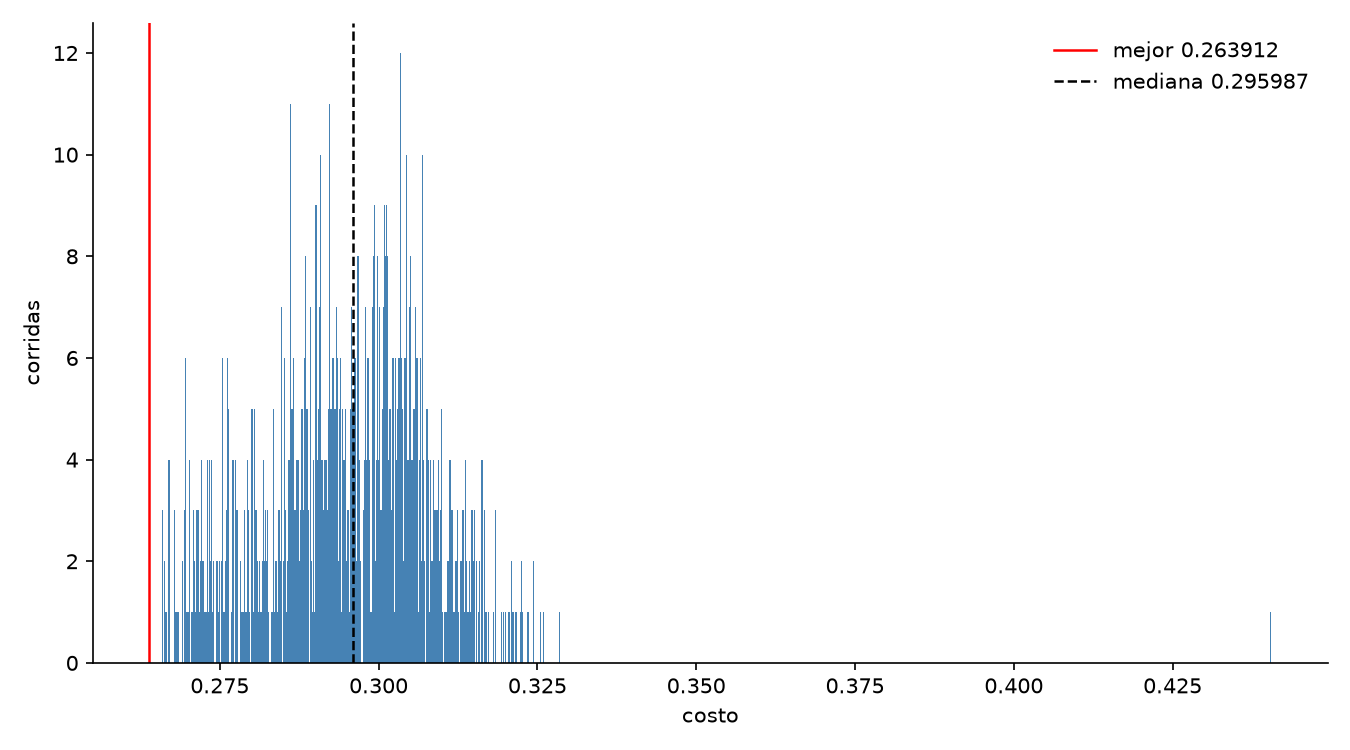
\includegraphics[width=1\linewidth]{figures/seeds40-BTS-false-dist.png}
    \caption{Histograma de 1000 corridas para 40 ciudades sin b\'usqueda binaria}
\end{figure}

El histograma generado parece tener una distribuci\'on normal. \\

\textbf{150 ciudades.} Mismos parámetros y misma semilla maestra. Las 1000 corridas tomaron \textbf{851.7~s} en total (1.17 corridas/s). El mejor costo fue \textbf{0.17462412491928164}, alcanzado por la semilla \inlinecode{-3342339423981252473}.

\begin{center}
    \small
    \begin{tabular}{lr}
        \hline
        Factibles & 2/1000 (0.2\%)\\
        Mejor & 0.17462412\\
        Mediana & 0.17995192\\
        Promedio & 0.17995192\\
        Peor & 0.18527972\\
        Desviación estándar & 0.00753465\\
        \hline
    \end{tabular}
\end{center}

\begin{figure}[H]
    \centering
    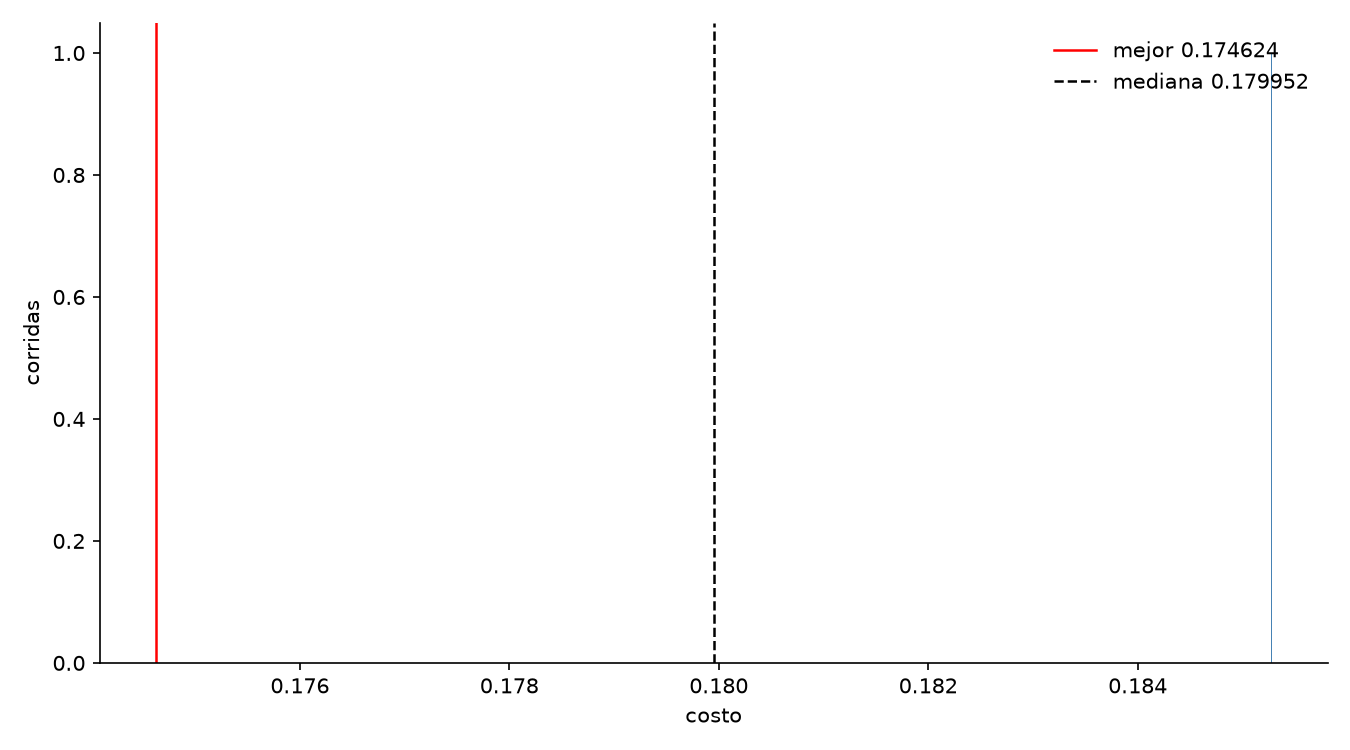
\includegraphics[width=1\linewidth]{figures/seeds150-BTS-false-dist.png}
    \caption{Histograma de 1000 corridas para 150 ciudades sin b\'usqueda binaria}
    \label{fig:placeholder}
\end{figure}

Para que el histograma tenga sentido visual, s\'olo toma en cuenta soluciones factibles. Para esta instancia, tan s\'olo dos soluciones lograron factibilidad,  y son precisamente la mejor, marcada en rojo, y la peor, marcada en azul.\\

Como se puede observar, la instancia de 40 ciudades tuvo un \textit{performance} decente. No obstante, la instancia de 150 ciudades tuvo un porcentaje de factibilidad en sus soluciones finales que no es aceptable. Vale la pena señalar que las estadísticas de la instancia de 150 ciudades se calculan sobre únicamente dos corridas factibles, por lo que su mediana, promedio y desviación estándar no describen el comportamiento del algoritmo, sino solo esas dos corridas. Cuando menos este resultado nos deja ver que en efecto la heur\'istica permite soluciones infactibles.


\subsection{Con búsqueda binaria para la temperatura}

Después, se probó activando la búsqueda binaria para la temperatura con el objetivo de comparar las soluciones obtenidas cuando se aplica esta técnica.\\

\textbf{40 ciudades.} Parámetros idénticos a los del experimento anterior, con la única diferencia de \inlinecode{searchTemperature = true}; misma semilla maestra \inlinecode{-5926462348639063530}. Las 1000 corridas tomaron \textbf{319.3~s} en total (3.13 corridas/s). El mejor costo fue \textbf{0.26381952559689636}, alcanzado por la semilla \inlinecode{811391249151273594}.

\begin{center}
    \small
    \begin{tabular}{lr}
        \hline
        Factibles & 1000/1000 (100.0\%)\\
        Mejor & 0.26381953\\
        Mediana & 0.29370696\\
        Promedio & 0.29242460\\
        Peor & 0.33077813\\
        Desviación estándar & 0.01319523\\
        \hline
    \end{tabular}
\end{center}


\begin{figure}[H]
    \centering
    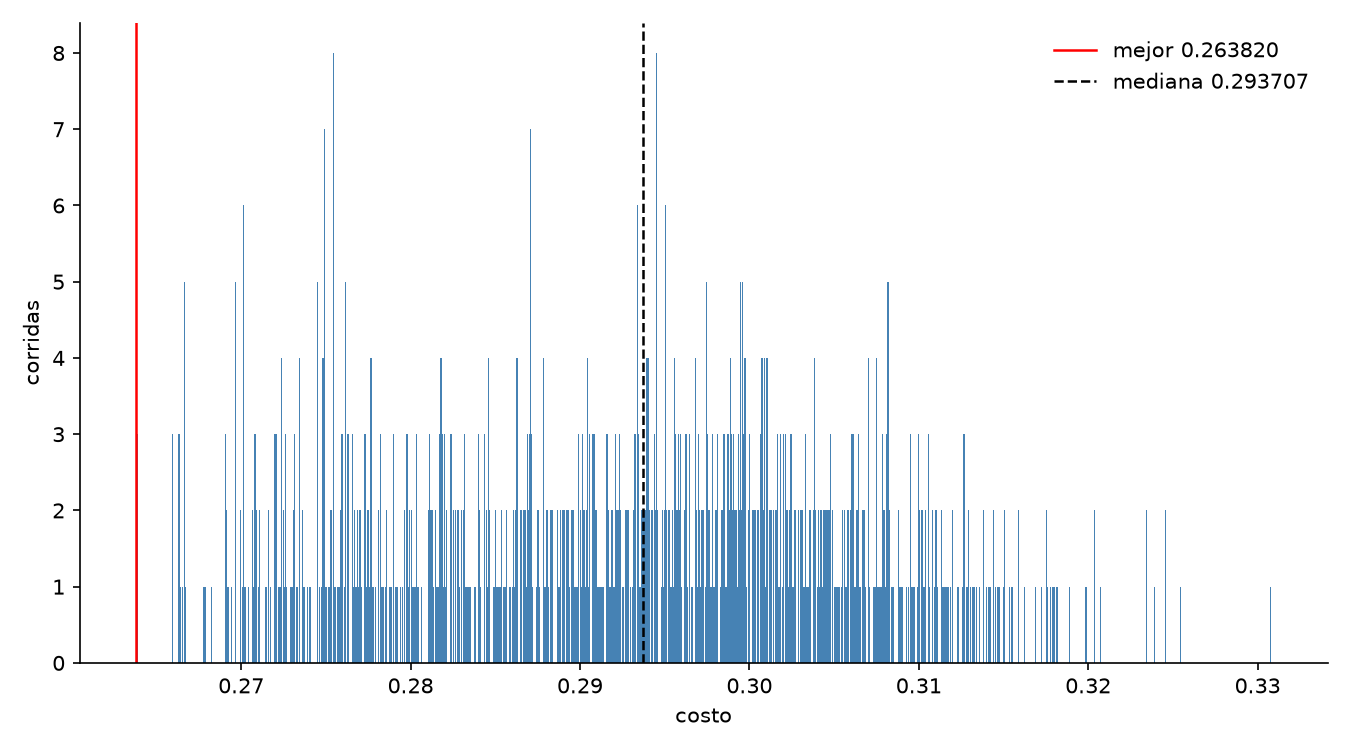
\includegraphics[width=1\linewidth]{figures/seeds40-BTS-true-dist.png}
    \caption{Histograma de 1000 corridas para 40 ciudades con b\'usqueda binaria}
    \label{fig:placeholder}
\end{figure}

El histograma revelado es en realidad muy parecido al del experimento anterior. Luce m\'as ancho porque la peor soluci\'on ya no se aleja tanto de la media. Cabe destacar que tanto la mediana como la mejor soluci\'on mejoraron ligeramente. De hecho, la mejor soluci\'on es la misma que la que se ver\'a en el siguiente experimento.\\


\textbf{150 ciudades.} Mismos parámetros y misma semilla maestra. Las 1000 corridas tomaron \textbf{1051.0~s} en total (0.95 corridas/s). El mejor costo fue \textbf{0.14246516817199148}, alcanzado por la semilla \inlinecode{-8843239329432448181}.

\begin{center}
    \small
    \begin{tabular}{lr}
        \hline
        Factibles & 769/1000 (76.9\%)\\
        Mejor & 0.14246517\\
        Mediana & 0.17449250\\
        Promedio & 0.17502456\\
        Peor & 0.50538887\\
        Desviación estándar & 0.01524970\\
        \hline
    \end{tabular}
\end{center}

\begin{figure}[H]
    \centering
    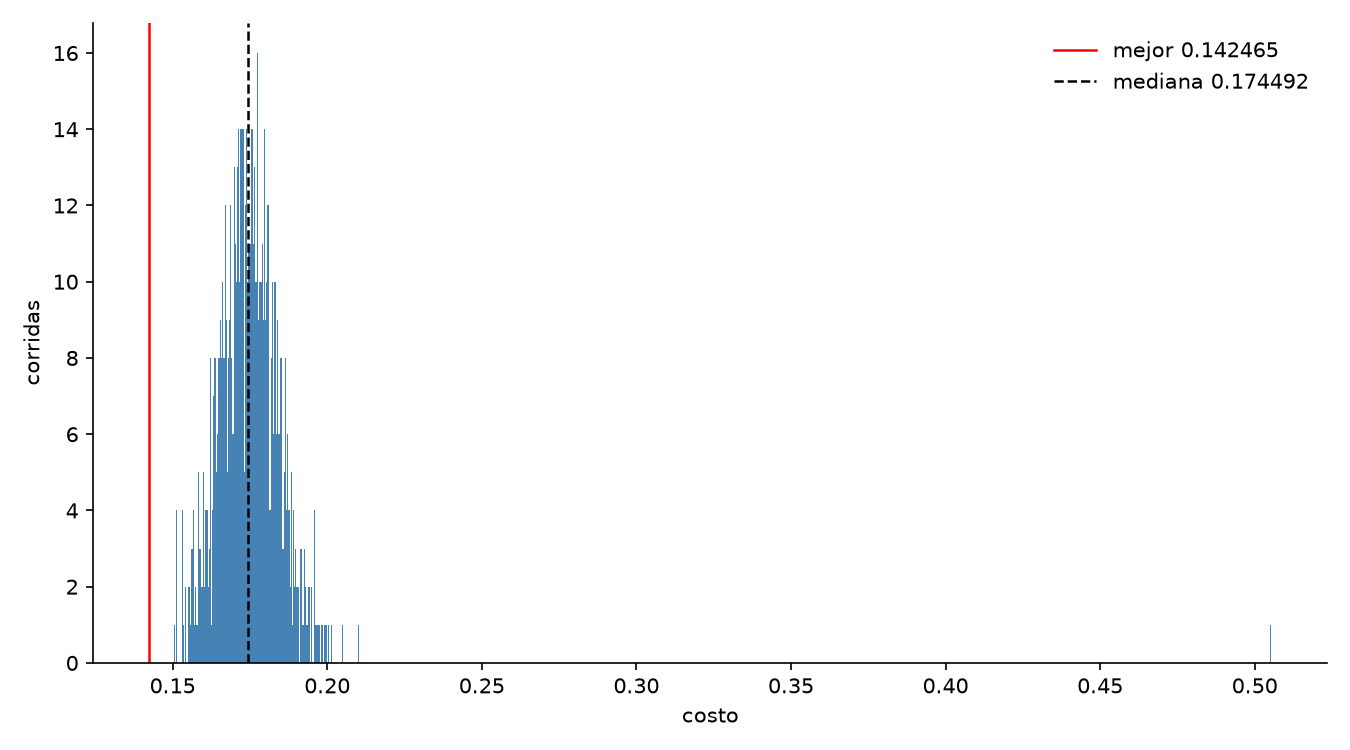
\includegraphics[width=1\linewidth]{figures/seeds150-BTS-true-dist.png}
    \caption{Histograma de 1000 corridas para 40 ciudades con b\'usqueda binaria}
    \label{fig:placeholder}
\end{figure}

Ahora en ambos casos logramos una distribuci\'on normal. \\

La búsqueda binaria aumentó significativamente el porcentaje de factibilidad: de 97.3\% a 100\% en la instancia de 40 ciudades, y de 0.2\% a 76.9\% en la de 150. Es indispensable tener un alto porcentaje de factibilidad; al menos un 80\%. De otra manera, estamos generando soluciones inexistentes y que en la práctica no sirven de nada. El costo de esa confiabilidad es tiempo: las mismas 1000 corridas pasaron de 238.7~s a 319.3~s en la instancia de 40 ciudades, y de 851.7~s a 1051.0~s en la de 150, ya que calcular $T_0$ consume evaluaciones antes de que empiece el enfriamiento propiamente dicho.

\subsection{2-opt}

Finalmente se sustituyó el operador de vecindad por la reversión de segmento descrita en la Sección~\ref{sec:heuristica}, y se reajustaron los parámetros del enfriamiento.\\

\textbf{40 ciudades.} Parámetros: $T_0 = 500000$, $\varphi = 0.995$, $L = 4000$, $\varepsilon = 10^{-9}$, cota de intentos por lote $= 6000$, cota global $= 10^{8}$, $P = 0.993$, \inlinecode{searchTemperature = true}; semilla maestra \inlinecode{-1417975048879117167}, 24 hilos. Las 1000 corridas tomaron \textbf{831.0~s} en total (1.20 corridas/s). El mejor costo fue \textbf{0.26381952559689636}, alcanzado por la semilla \inlinecode{130071593650909319}.

\begin{center}
    \small
    \begin{tabular}{lr}
        \hline
        Factibles & 1000/1000 (100.0\%)\\
        Mejor & 0.26381953\\
        Mediana & 0.26389366\\
        Promedio & 0.26446397\\
        Peor & 0.26590735\\
        Desviación estándar & 0.00081647\\
        \hline
    \end{tabular}
\end{center}

\begin{figure}[H]
    \centering
    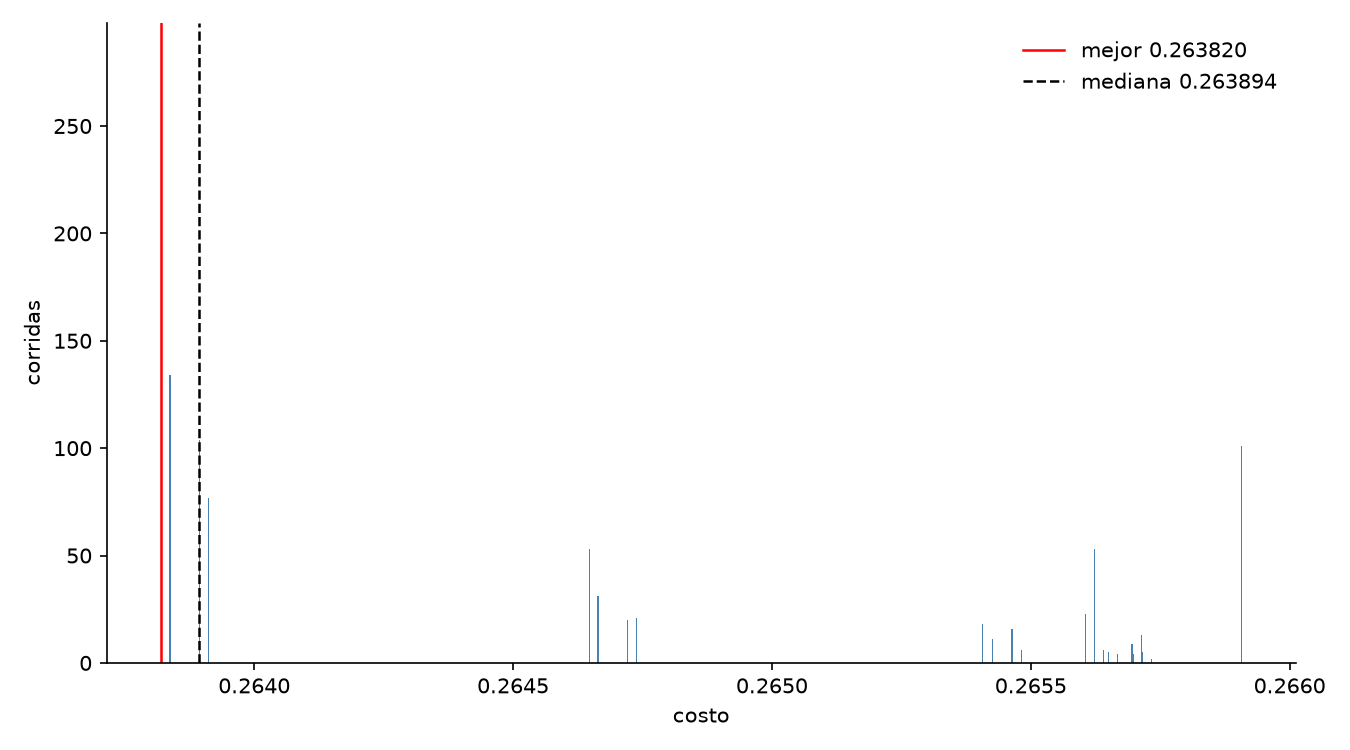
\includegraphics[width=1\linewidth]{figures/seeds40-dist.png}
    \caption{Histograma de 1000 corridas para 40 ciudades con 2-opt}
    \label{fig:placeholder}
\end{figure}


\textbf{150 ciudades.} Mismos parámetros y misma semilla maestra, con 20 hilos. Las 1000 corridas tomaron \textbf{2580.0~s} en total (0.39 corridas/s). El mejor costo fue \textbf{0.13623807950353167}, alcanzado por la semilla \inlinecode{6091304898049588117}.

\begin{center}
    \small
    \begin{tabular}{lr}
        \hline
        Factibles & 1000/1000 (100.0\%)\\
        Mejor & 0.13623808\\
        Mediana & 0.13726826\\
        Promedio & 0.13748888\\
        Peor & 0.14218576\\
        Desviación estándar & 0.00096541\\
        \hline
    \end{tabular}
\end{center}

\begin{figure}[H]
    \centering
    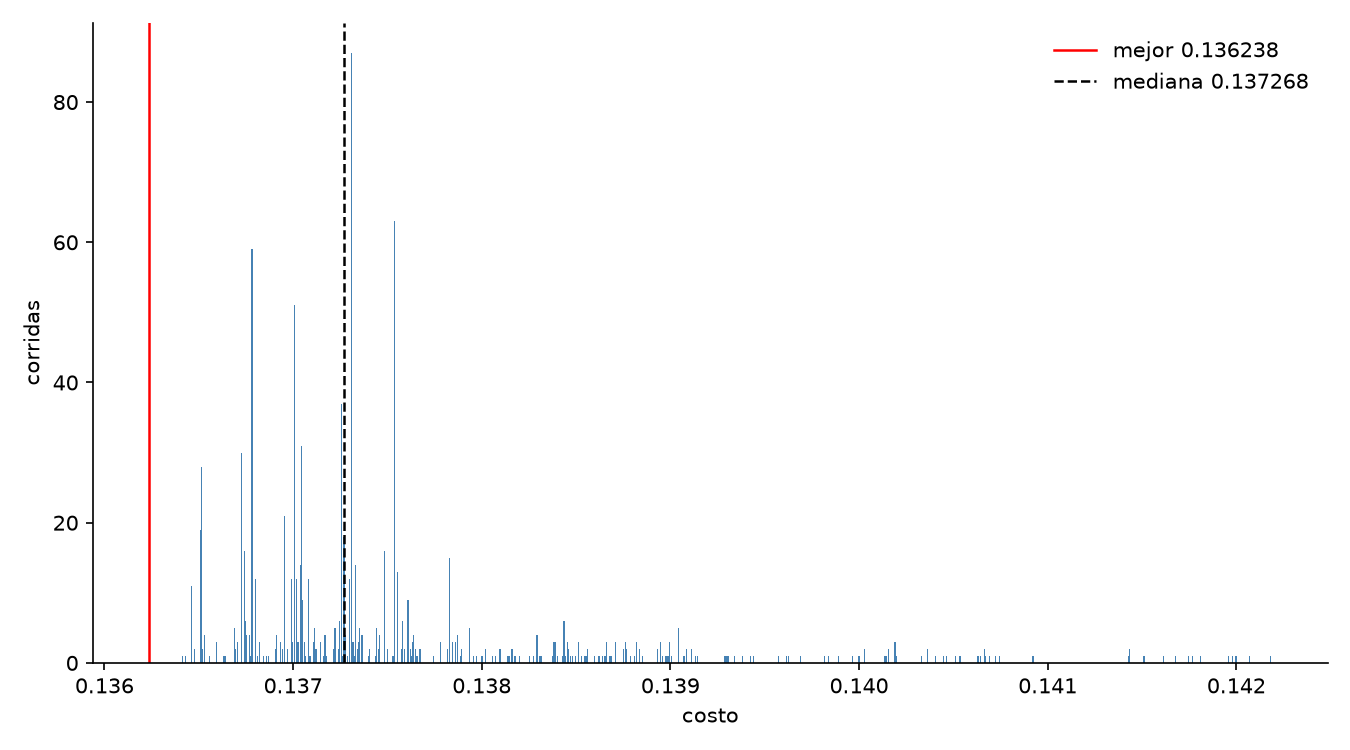
\includegraphics[width=1\linewidth]{figures/seeds150-dist.png}
    \caption{Histograma de 1000 corridas para 150 ciudades con 2-opt}
    \label{fig:placeholder}
\end{figure}

Pareciera que ambos histogramas tienen datos faltantes, pero en realidad lo que sucede es que muchas de las soluciones producidas a partir de distintas semillas convergieron en exactamente los mismos resultados, particularmente en la instancia de tamaño 40.\\

La calidad de las soluciones mejora tremendamente cuando aplicamos la optimización. Por primera vez logramos costos inferiores a .14. La desviación estándar es el indicador más claro del cambio: pasó de 0.01319523 a 0.00081647 en la instancia de 40 ciudades, y de 0.01524970 a 0.00096541 en la de 150, un orden de magnitud menos en ambos casos. Ya no se trata solo de que la mejor corrida sea mejor, sino de que la peor corrida de este experimento (0.26590735 y 0.14218576 respectivamente) es comparable con la \emph{mejor} corrida de los experimentos anteriores.\\

Para la instancia de 40 ciudades, el mejor costo logrado es de 0.26381952559689636, en tan solo 3.7 segundos por ejecución individual. En el barrido de 1000 semillas, el número de semillas diferentes que reprodujeron este resultado fue de 284, lo que representa el 28.4\% del total. Esto nos lleva a sospechar fuertemente que es muy probable que hayamos encontrado el óptimo de entre todo el espacio de búsqueda. Aún así, resulta imposible asegurarlo sin verificar exhaustivamente que no existe una mejor solución.\\

En la instancia de 150 ciudades, el mejor resultado encontrado no es tan común como en la de 40 ciudades. En el barrido de 1000 semillas, tan sólo 5 lograron alcanzar ese resultado. De todas formas, en el histograma se observa que la media de soluciones es de 0.13748888, a una distancia de apenas 0.9\% del mejor costo encontrado.\\

\subsection{Costo vs Temperatura}

\begin{figure}[H]
    \centering
    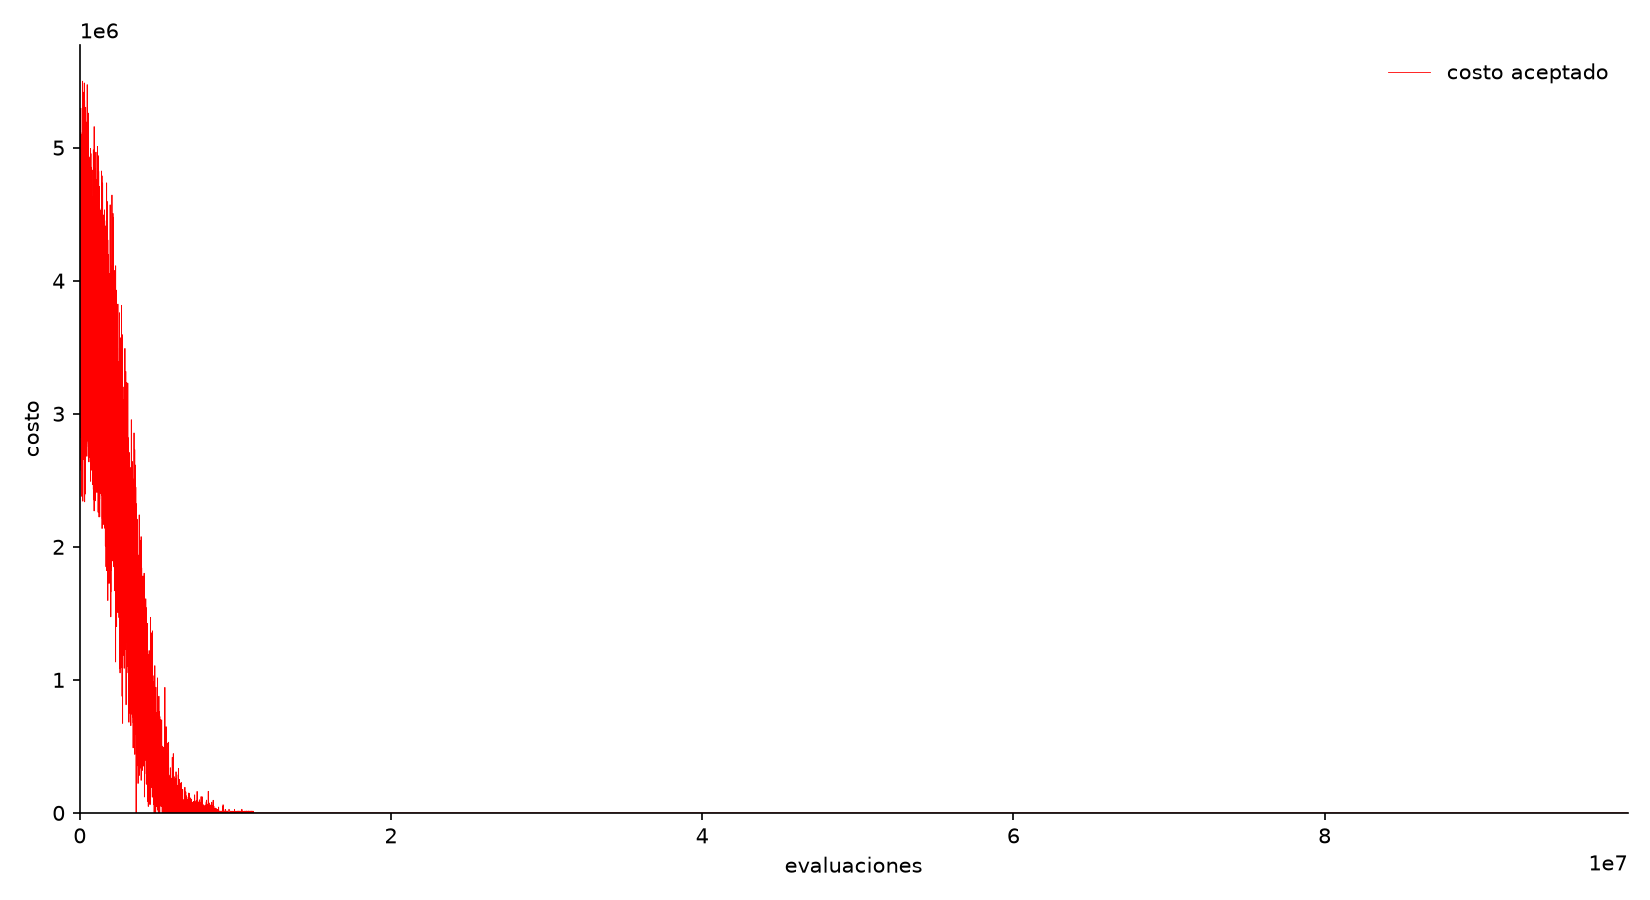
\includegraphics[width=1\linewidth]{figures/40.png}
    \caption{Gr\'afica de costos aceptados vs temperatura para 40 ciudades}
    \label{fig:placeholder}
\end{figure}

En la de 150 ciudades se aprecia de mejor manera c\'omo es que la curva al inicio sube ligeramente para despu\'es caer, y conforme cae, el rango aceptado se va estrechando.

\begin{figure}[H]
    \centering
    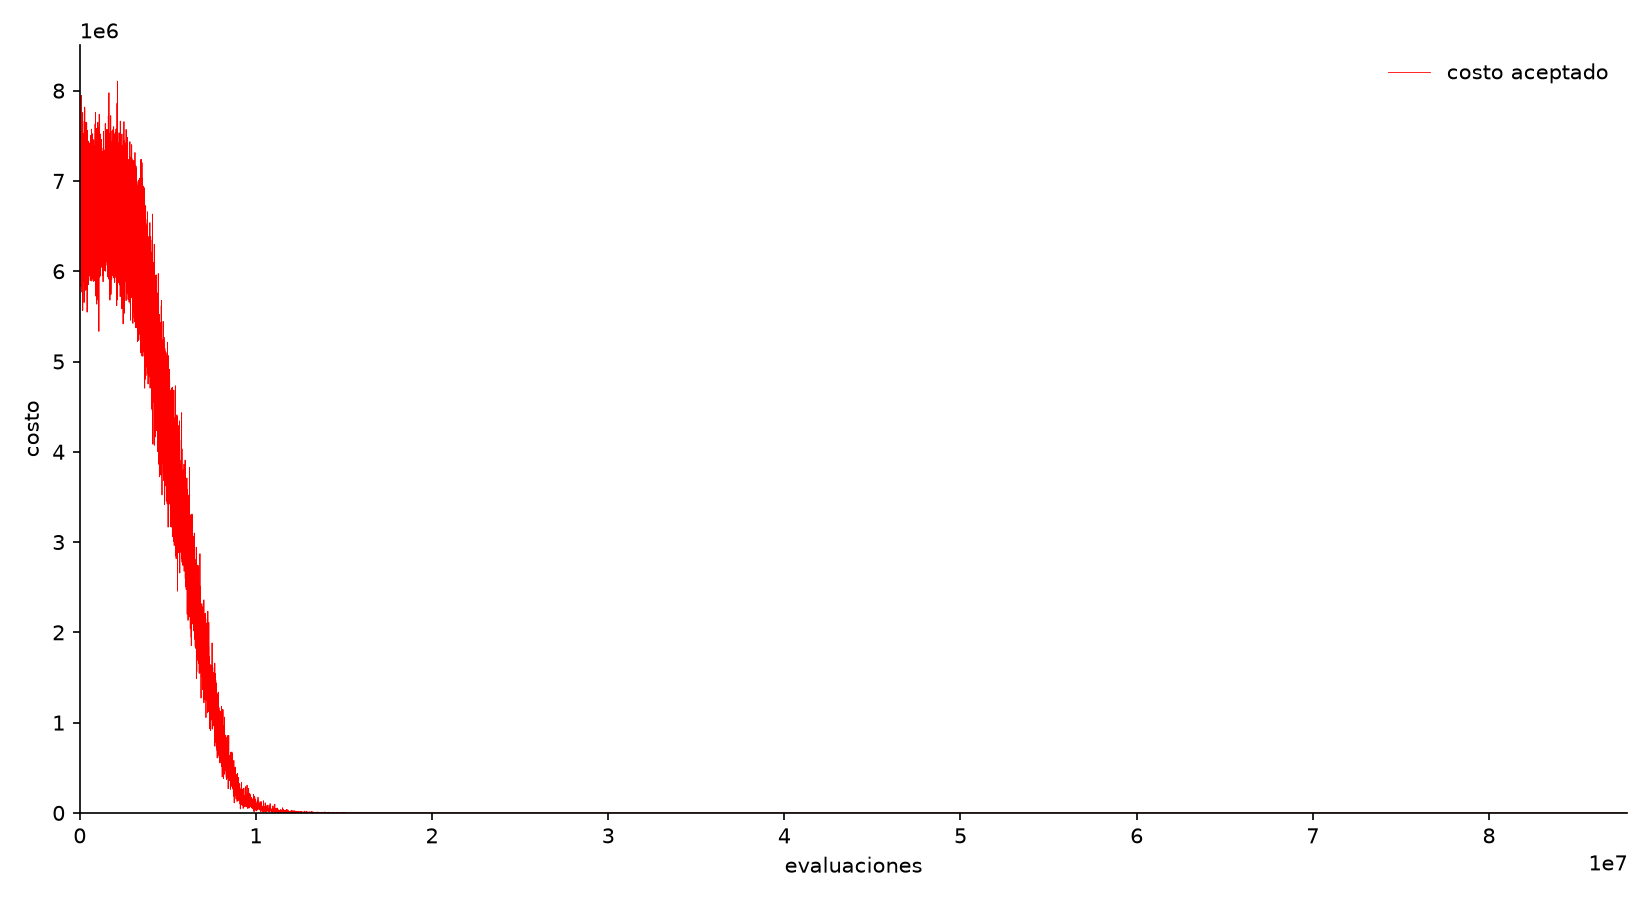
\includegraphics[width=1\linewidth]{figures/150.png}
    \caption{Gr\'afica de costos aceptados vs temperatura para 150 ciudades}
    \label{fig:placeholder}
\end{figure}

Para observar de forma gr\'afica el comportamiento de la heur\'istica, se realizaron gr\'aficas de los costos aceptados en funci\'on de la temperatura. Guardan cierta similitud con las encontradas en la literatura, aunque la curva que generan es bastante empinada. Podemos ver que al inicio sucede la etapa de exploraci\'on, donde se permite que las soluciones empeoren, para luego llegar a valores muy bajo y explotar las mejores soluciones encontradas. La escala ni siquiera nos permite apreciar la l\'inea roja representando el costo.

\begin{figure}[H]
    \centering
    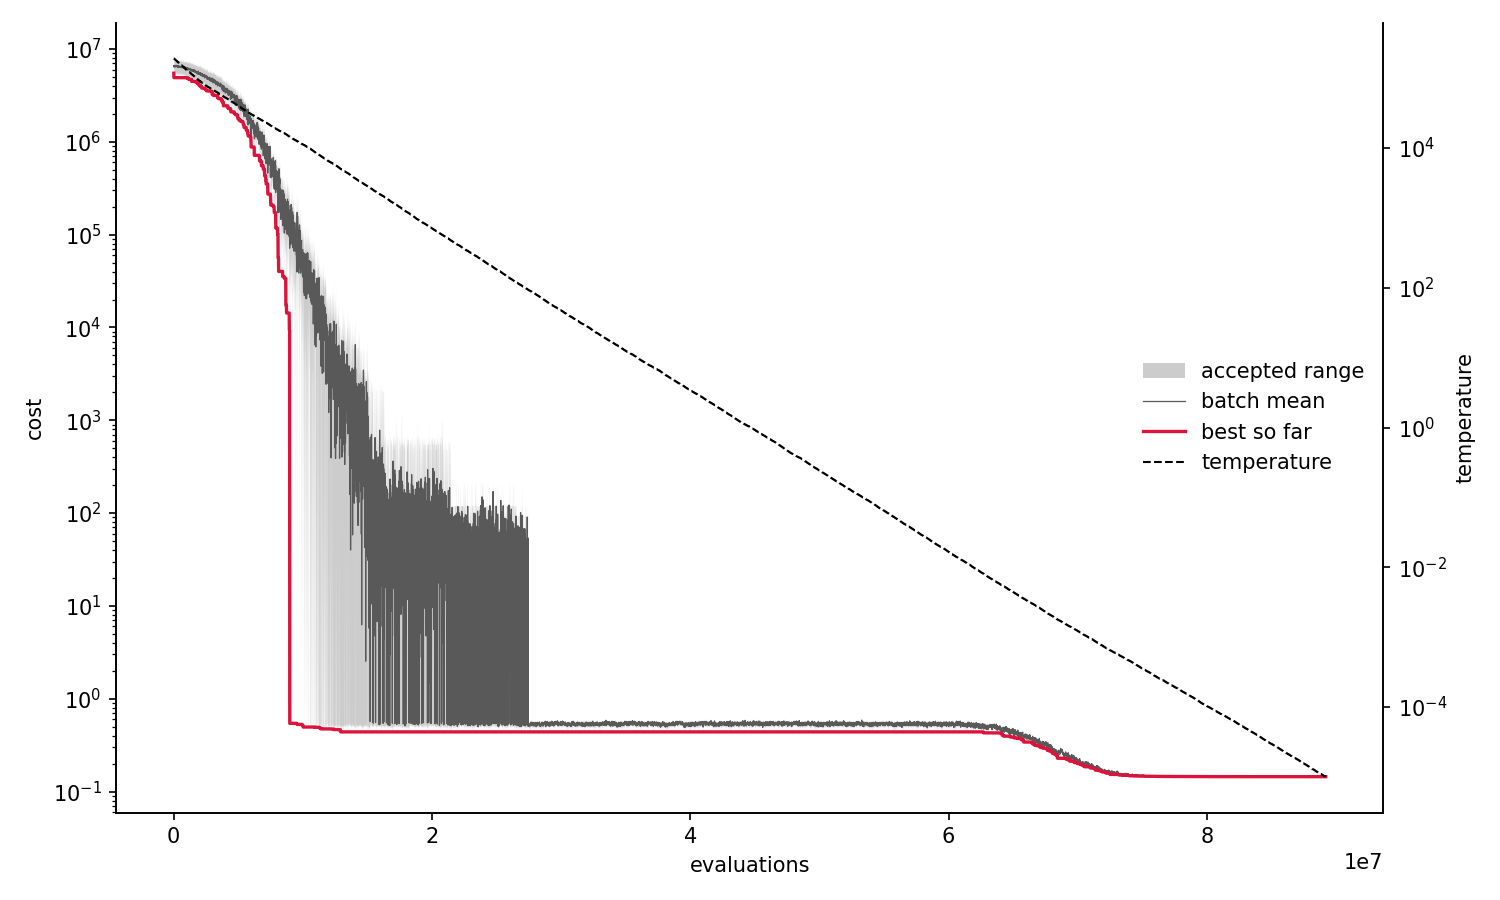
\includegraphics[width=1\linewidth]{figures/batchmean.png}
    \caption{Evolución del costo aceptado por lote y de la temperatura a lo largo de una corrida completa sobre 150 ciudades}
    \label{fig:placeholder}
\end{figure}

Tambi\'en se grafic\'o el an\'alisis de costos contra evaluaciones. Este an\'alsis toma en cuenta la media de costo por lote, donde se ve de forma clara c\'omo al inicio la factibilidad de las soluciones no es buena, y llega un punto en el que la heur\'istica descarta por completo costos menores a $1$. Ya m\'as hacia el final, vemos que hay una bajada suave a costos a\'un menores, permitidos por tener una \'epsilon de terminaci\'on muy cercana a cero.

\subsection{Mapas}



\begin{figure}[H]
    \centering
    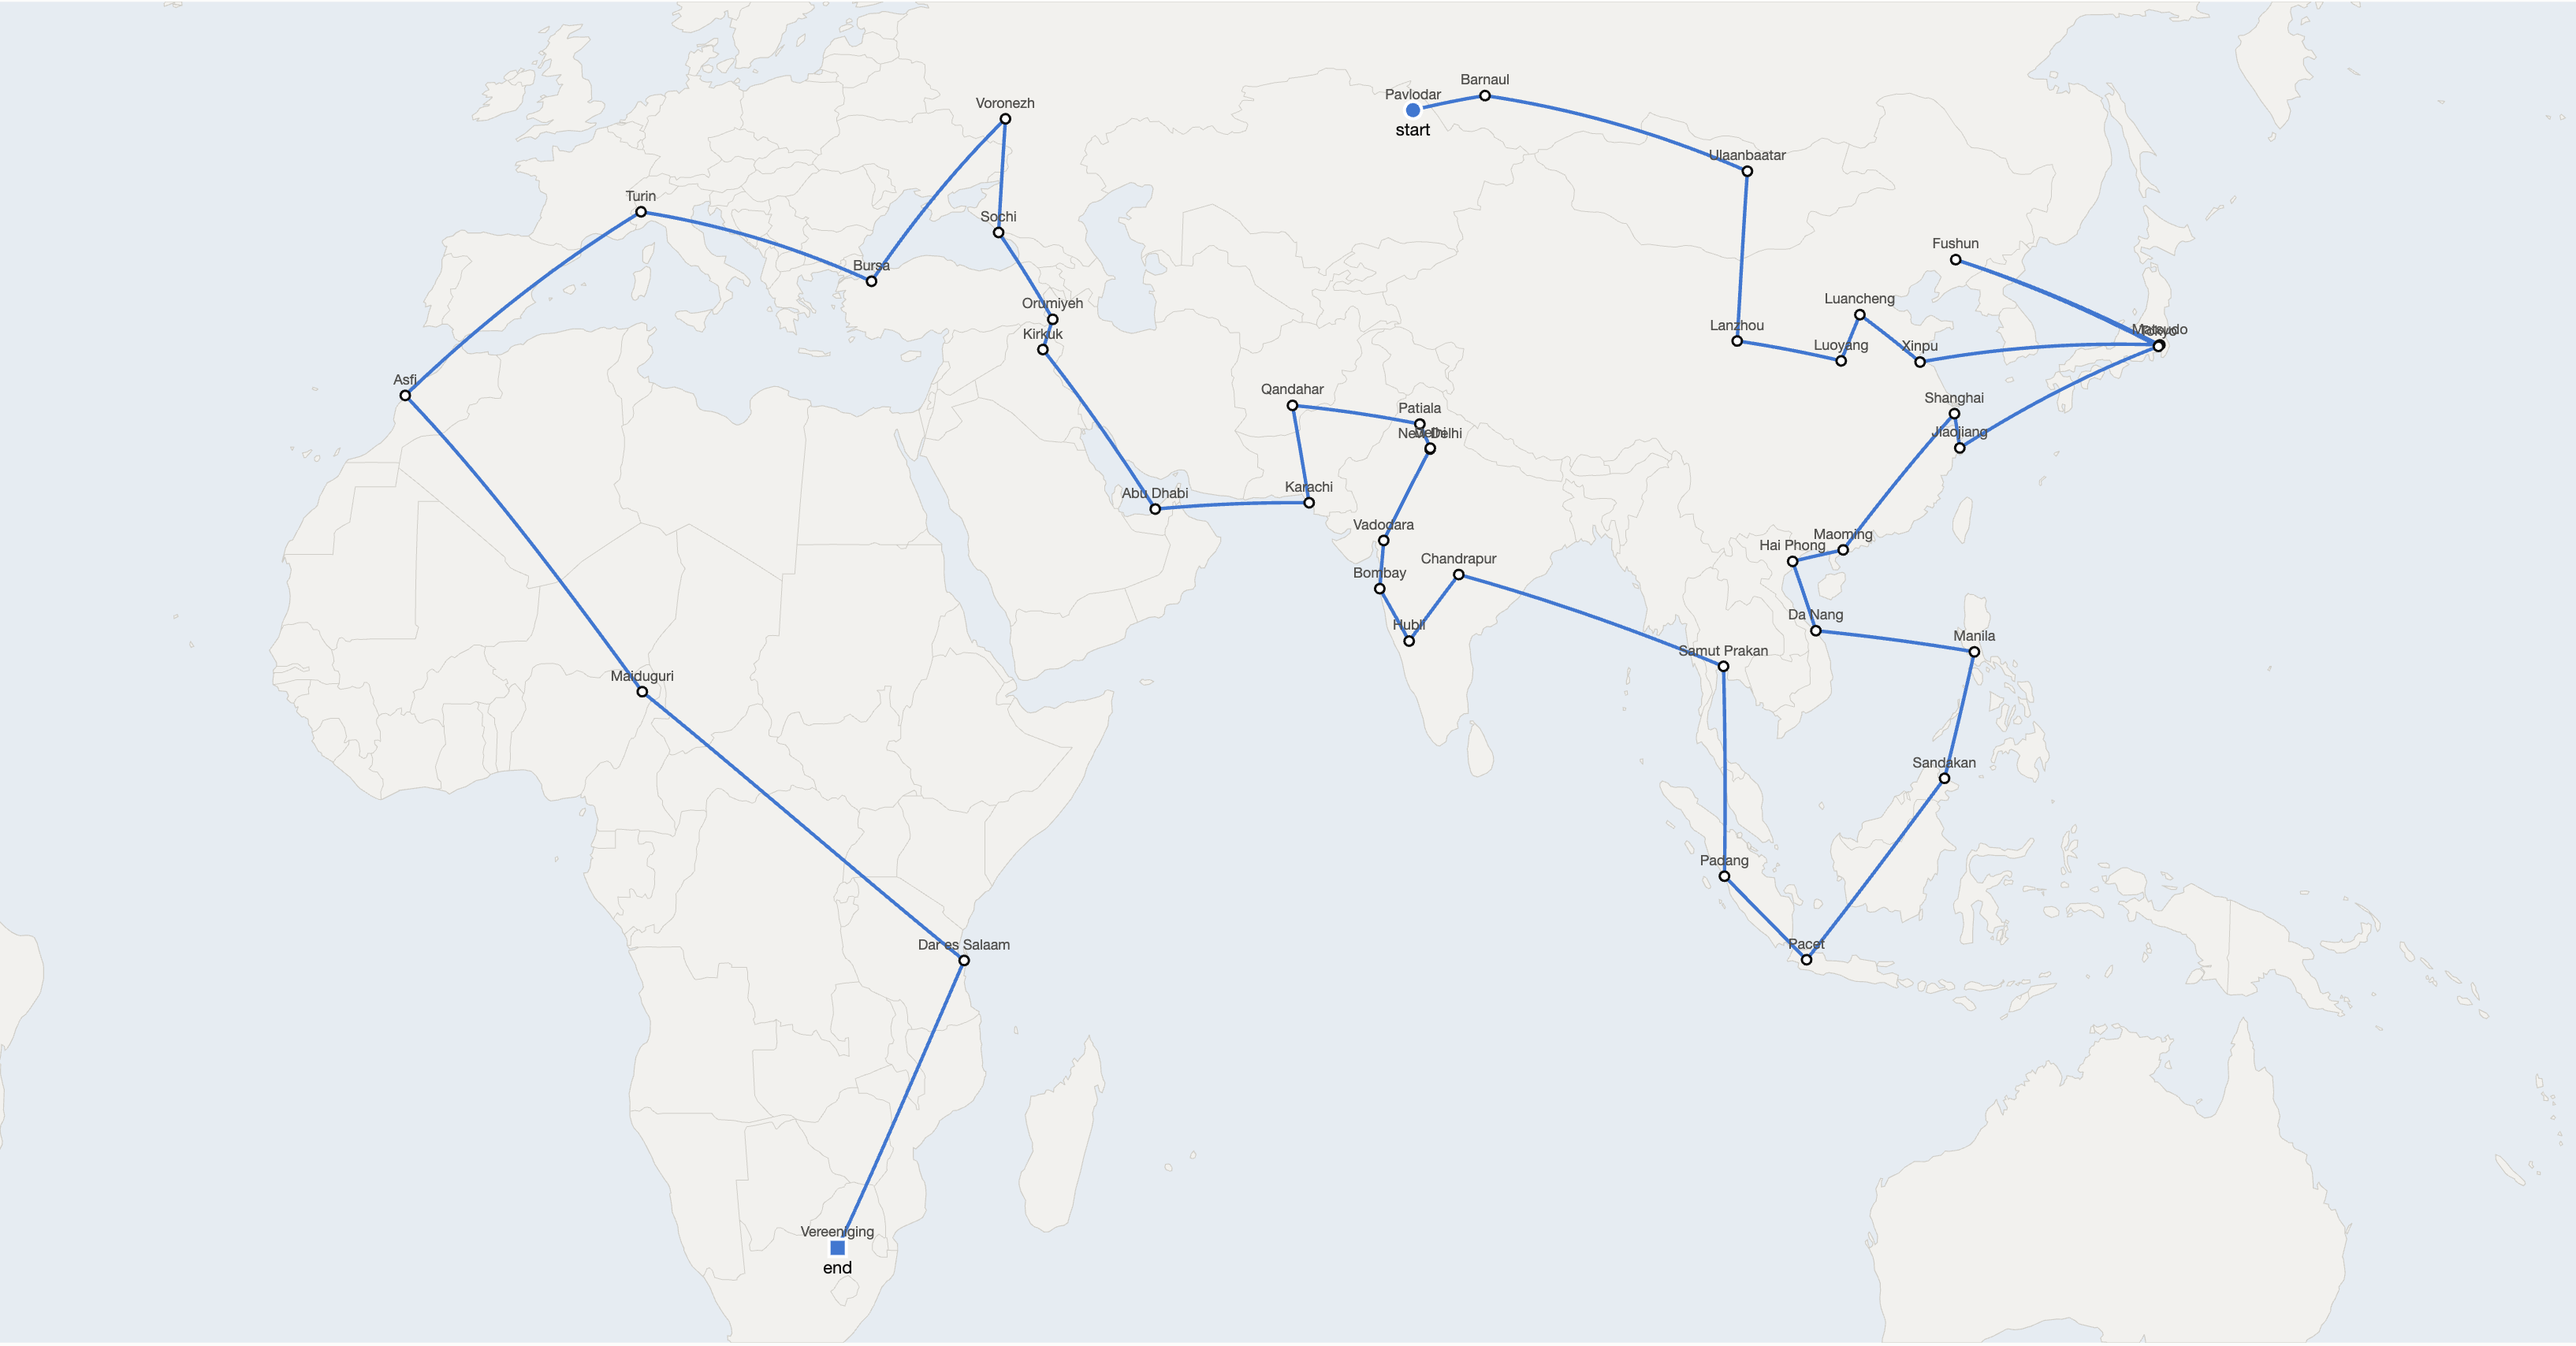
\includegraphics[width=1\linewidth]{figures/mapa-40.png}
    \caption{Mapa de la mejor ruta encontrada para 40 ciudades}
    \label{fig:placeholder}
\end{figure}

\begin{figure}[H]
    \centering
    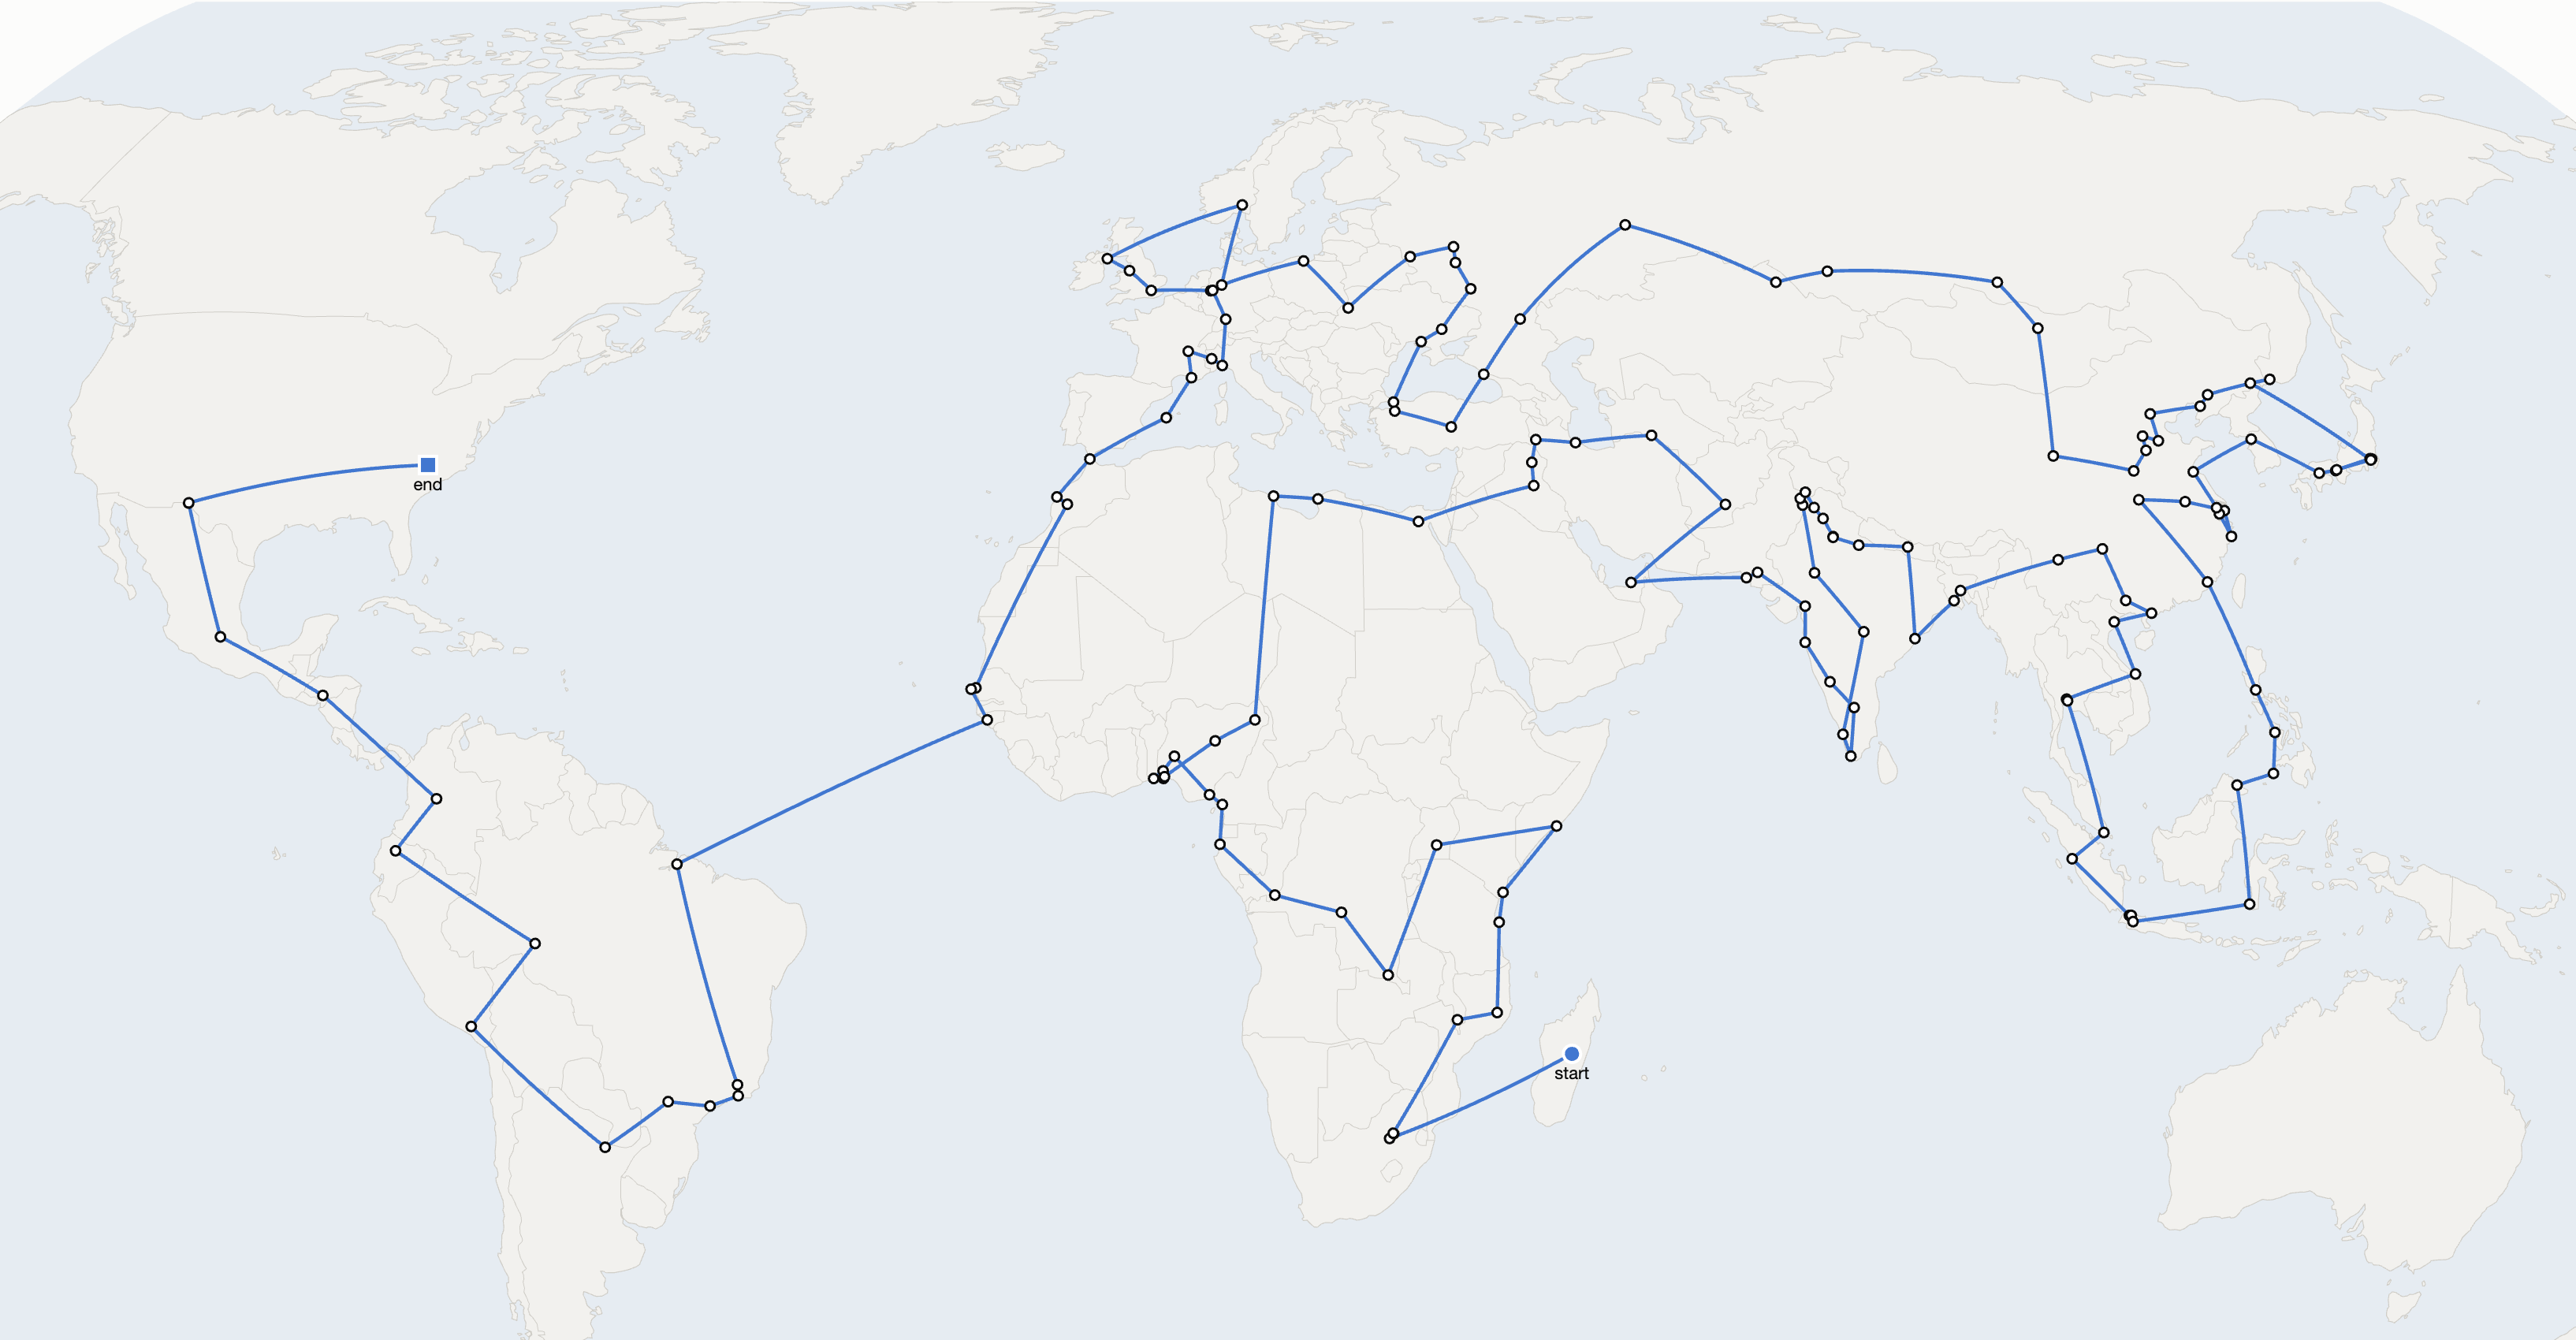
\includegraphics[width=1\linewidth]{figures/mapa-150.png}
    \caption{Mapa de la mejor ruta encontrada para 40 ciudades}
    \label{fig:placeholder}
\end{figure}


Por \'ultimo, la visualizaci\'on en mapa de la trayectoria entre ciudades nos deja ver que geom\'etricamente, las mejores soluciones obtenidas tienen sentido. Existen cruces m\'inimos entre aristas, y es posible que aquellos que s\'i se presentan sean imposibles de eliminar en esa configuiraci\'on debido a las caracter\'isticas espec\'ificas de las instancias y las conexiones inexistentes entre ciudades.\\





% ==============================================================================
% 7. CONCLUSIONES Y TRABAJO FUTURO
% ==============================================================================
\section{Conclusiones}

Los resultados presentados mantuvieron los mismos par\'ametros de tamaño de lote, temperatura inicial, final, factor de enfriamiento, aceptaci\'on objetivo y n\'umero de intentos permitidos. Para hacer un an\'alsis completo, se deber\'ian de habe reportado las diferencias halladas entre estos par\'ametros. Aquellos que se usaron para hallar las soluciones fueron elegidos porque en la prueba y error, resultaron mejores. En general, factores como la tasa de enfriamiento producen mejores soluciones mientras m\'as cercana a 1 sea. Sin embargo, este comportamiento no es una regla; hab\'ia veces donde las soluciones no mejoraban, o incluso empeoraban. Esto suced\'ia igual para el resto de par\'ametros.\\

En cuanto a lo s\'i reportado, vemos que la implementaci\'on de la b\'usqueda binaria fue fundamental para lograr resultados confiables. Para la mejora de calidad en los resultados en s\'i, lo que result\'o \'util fue 2-opt. Es importante revisar resultados con muestras lo suficientemente grandes y con distintos tamaños de instancia para detectar anomal\'ias y patrones en el comportamiento. \\

        
    \subsection*{Conclusiones personales}
    Siendo sincera, titubeé acerca de dejar inscrita esta materia. No tenía confianza en mí misma para llegar a soluciones decentes. Este proyecto ha probado lo contrario; terminé dedicándole muchas más horas de lo que tenía planeado. Lo mejor de todo es que conforme más avanzaba con el mismo, más divertido resultaba ver mis resultados e intentar mejorarlos. Hacía tiempo no me resultaba satisfactorio hacer un proyecto académico.\\

    Sin duda uno de los componentes fundamentales para evitar caer en la frustración dueanre el desarrollo fueron mis compañeros de grupo. Una vez con la heurística implementada, surgió una carrera por ver quién lograba mejores resultados. Esta competencia en ningún momento fue destructiva. Al contrario, se fomentó la mejora y la colaboración continua. Esta fue una pequeña muestra de cómo la colaboración científica da sus frutos, y sin duda me invita a querer reptir la dinámica en el futuro.

% ==============================================================================
% BIBLIOGRAFÍA
% ==============================================================================

\printbibliography

%----------------------------------------------------------

\end{document}